%==============================================================================
%  §3  Problem Definition                                          [owner: A1]
%  Source: v8 §3 (sec:problem, v8:90-341), restructured into six subsections.
%  Relocated in:  def:imbalance + eq:imbalance_ratio (from v8 §4)
%                 asm:margin    + eq:margin_assumption (from v8 §4)
%                 asm:hbm       + tab:assumption_chain (from v8 app:hbm)
%                 eq:entrywise                         (from v8 §5)
%                 the distance operator B = H D H      (from v9 sec:main-dist)
%
%  [Reviewer Note (v9 refine pass): subsections 2.1-2.5 deleted; the section now
%  runs as one narrative, with the former headings carried by transition
%  sentences.  Five headings over eight pages of setup announced structure the
%  reader could already see, and each one restarted the prose.  The three
%  \begin{definition} environments (imbalance, margin, coherence) are unwrapped
%  into running text with their numbered equations untouched, so eta and rho now
%  arrive where they are first used rather than as formal declarations; external
%  \Cref{def:*} references were retargeted to \eqref{eq:*}.  The assumption
%  environments are NOT dissolved -- they are cited as hypotheses inside
%  thm:main-sim and must stay referenceable.]
%==============================================================================
\section{Problem Definition}\label{sec:problem}

Our starting point is purely topological. Let $\mathcal{T} = (V, E)$ be a rooted
latent binary phylogenetic tree whose vertex set $V = \mathcal{X} \cup \mathcal{H}$
splits into $m$ observed terminal leaves $\mathcal{X} = \{x_1, \dots, x_m\}$ and
$m-1$ unobserved internal ancestral nodes $\mathcal{H} = \{h_1, \dots, h_{m-1}\}$,
among them a distinguished root $r \in \mathcal{H}$ \cite{aizenbud2023spectral}.
The two edges descending from $r$ define the \emph{primary split} of the tree:
the leaf set $\mathcal{X}$ is partitioned into the two subtrees hanging off the
root.

We call each side of this split a \emph{clan}
\cite{aizenbud2023spectral, wilkinson2007clades, semple2003phylogenetics}:
topologically, a clan is the leaf set of one of the two root subtrees, the
maximal monophyletic group induced by the root edge. The term is the unrooted
analogue of a clade \cite{wilkinson2007clades}, so the root-split bipartition is
precisely a pair of complementary clans, consistent with the unrooted similarity
matrix we analyze. This single bipartition $\mathcal{X} = A \cup B$, rather than
the full branching pattern of $\mathcal{T}$, is the object we set out to recover;
resolving it is the top-down step from which the remaining tree structure follows
recursively. Throughout, we order the leaves along the split so that leaves $1$
through $a$ form clan $A$ and leaves $a+1$ through $m$ form clan $B$, which lets us
speak of a clan equivalently as a contiguous block of indices.

The bridge from this topology to linear algebra is the population similarity
matrix. Let $S \in \R^{m \times m}$ be the symmetric matrix of pairwise
similarities over the leaves $\mathcal{X}$, normalized so that $S_{ii} = 1$
\cite{aizenbud2023spectral}. Under the clan ordering, the primary split becomes an
algebraic object: the within-clan pairs occupy the two diagonal blocks of $S$, and
the cross-clan pairs its off-diagonal block. Writing $a=|A|$, $b=|B|$, and
$J_{a\times b}$ for the all-ones block, the constant cross-clan boundary developed
below gives $S$ and its combinatorial Laplacian $L=D-S$ the block form shown in
\Cref{fig:structural_split_balanced}. The generative model below makes this matrix
concrete, turning branch lengths and the substitution process into the block
structure of $S$.

\begin{figure}[t]
\centering
\small

\begin{minipage}[c]{0.5\textwidth}
\centering
\resizebox{\linewidth}{!}{%
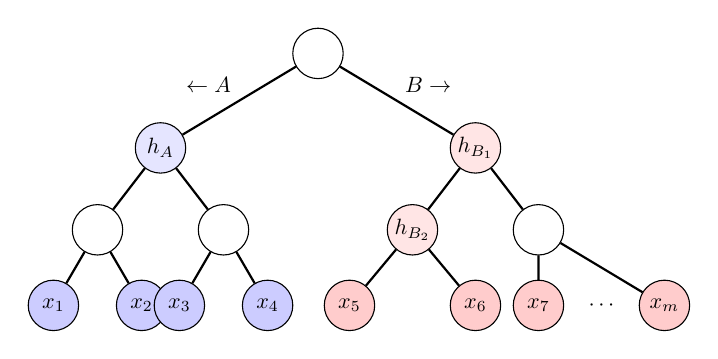
\begin{tikzpicture}[
    scale=0.8,
    every node/.style={transform shape},
    internal/.style={circle, draw, minimum size=8mm, inner sep=1pt},
    leaf/.style={circle, draw, minimum size=8mm, inner sep=1pt, fill=blue!20},
    leafright/.style={circle, draw, minimum size=8mm, inner sep=1pt, fill=red!20}
]
    % Level 0: Root
    \node[internal] (root) at (0, 4) {};

    % Level 1: Clan Roots
    \node[internal, fill=blue!10] (hA) at (-2.5, 2.5) {$h_A$};
    \node[internal, fill=red!10] (hB1) at (2.5, 2.5) {$h_{B_1}$};

    % Level 2: Internal nodes to maintain equal depth
    \node[internal] (l2_1) at (-3.5, 1.2) {};
    \node[internal] (l2_2) at (-1.5, 1.2) {};
    \node[internal, fill=red!10] (hB2) at (1.5, 1.2) {$h_{B_2}$};
    \node[internal] (l2_4) at (3.5, 1.2) {};

    % Level 3: Terminal Nodes (Leaves) at y=0
    % Clan A Leaves
    \node[leaf] (x1) at (-4.2, 0) {$x_1$};
    \node[leaf] (x2) at (-2.8, 0) {$x_2$};
    \node[leaf] (x3) at (-2.2, 0) {$x_3$};
    \node[leaf] (x4) at (-0.8, 0) {$x_4$};

    % Clan B Leaves
    \node[leafright] (x5) at (0.5, 0) {$x_5$};
    \node[leafright] (x6) at (2.5, 0) {$x_6$};
    \node[leafright] (x7) at (3.5, 0) {$x_7$};
    \node at (4.5, 0) {$\cdots$};
    \node[leafright] (xm) at (5.5, 0) {$x_m$};

    % Edges (Root to Level 1)
    \draw[thick] (root) -- (hA) node[midway, above left] {$\leftarrow A$};
    \draw[thick] (root) -- (hB1) node[midway, above right] {$B \rightarrow$};

    % Edges (Level 1 to Level 2)
    \draw[thick] (hA) -- (l2_1);
    \draw[thick] (hA) -- (l2_2);
    \draw[thick] (hB1) -- (hB2);
    \draw[thick] (hB1) -- (l2_4);

    % Edges (Level 2 to Level 3)
    \draw[thick] (l2_1) -- (x1);
    \draw[thick] (l2_1) -- (x2);
    \draw[thick] (l2_2) -- (x3);
    \draw[thick] (l2_2) -- (x4);

    \draw[thick] (hB2) -- (x5);
    \draw[thick] (hB2) -- (x6);
    \draw[thick] (l2_4) -- (x7);
    \draw[thick] (l2_4) -- (xm);

\end{tikzpicture}%
}
\vspace{2mm}
\subcaption{Balanced-Depth Clans $\mathcal{T}$}
\end{minipage}%
\hfill
\begin{minipage}[c]{0.45\textwidth}
\centering

\[
S=\begin{pmatrix} S_A & \bze J_{a\times b}\\ \bze J_{b\times a} & S_B\end{pmatrix}
\]
\vspace{1mm}
\subcaption{Matrix $S$ Structure}

\vspace{8mm}

\[
L=\begin{pmatrix} D_A-S_A & -\bze J_{a\times b}\\ -\bze J_{b\times a} & D_B-S_B\end{pmatrix}
\]
\vspace{1mm}
\subcaption{Laplacian $L$ Structure}

\end{minipage}

\vspace{4mm}
\caption{Visual topology of two lineage clans under a localized root split
boundary condition, maintaining the same depth but differing terminal node
counts. Shown alongside their corresponding population matrix block
configurations ($S$ and $L$ stacked vertically).}
\label{fig:structural_split_balanced}
\end{figure}

Branch lengths put a quantitative skin on the bare topology. Each edge
$(h, h') \in E$ carries a branch length $\tau_{hh'} \ge 0$ representing
evolutionary time. Absolute node times $\tau_h \ge 0$ are measured from the root,
with leaves fixed at $\tau = 0$, so $\tau_{hh'} = |\tau_h - \tau_{h'}|$. Running a
substitution process along these edges is what converts the tree into the
similarity matrix $S$.

\begin{assumption}[Generative model: GTR and log-det similarity]\label{asm:gtr}
Sequences of length $\ell$ over a $d$-character alphabet evolve along $\mathcal{T}$
under a \emph{General Time-Reversible} (GTR) rate matrix $Q \in \R^{d \times d}$
satisfying (i)~$Q_{ij}\ge0$ for $i\ne j$, (ii)~$\sum_j Q_{ij}=0$ for all $i$,
(iii)~a stationary distribution $\pi>0$ with $\pi Q=0$, and (iv)~$\mathrm{diag}(\pi)Q$
symmetric (reversibility). These imply $\mathrm{tr}(Q)<0$ with all eigenvalues
non-positive, and the substitution matrix along $(h,h')$ is
$P_{h|h'}=\exp(Q\,\tau_{hh'})$. The \emph{population similarity} between leaves
$i,j$ is the log-det similarity \cite{aizenbud2023spectral}
\begin{equation}\label{eq:similarity_gtr}
    S_{ij} = \exp\!\bigl(4\,\mathrm{tr}(Q)\,\tau_{ij}\bigr),
\end{equation}
where $\tau_{ij}$ is the depth of $\mathrm{MRCA}(i,j)$, a purely topological
quantity; \eqref{eq:similarity_gtr} thus maps the tree onto $S$, the first fully
linear-algebraic object of the paper. The empirical log-det estimator
$\hat S_{ij}$ concentrates around $S_{ij}$ at rate $\mathcal O(1/\sqrt\ell)$
\cite{aizenbud2023spectral}; the structural conditions that follow are stated
as properties of the population $S$, whose observable proxy is $\hat S$.
\end{assumption}

We now read the topology off the matrix. Since $\mathrm{tr}(Q)<0$,
\eqref{eq:similarity_gtr} makes $S_{ij}$ a decreasing function of the MRCA depth
$\tau_{ij}$, so leaves with a shallower common ancestor are more similar.
Within-clan pairs satisfy $\tau_{ij}<\tau_{\mathrm{root}}$ and therefore dominate
every cross-clan pair: the primary split appears as two strong diagonal blocks of
$S$ separated by a weaker off-diagonal block. Four conditions turn this depth
monotonicity into algebra: the molecular clock (\Cref{asm:clock}) collapses the
cross-clan block to a single baseline; the Constant Block Model
(\Cref{asm:cbm}) idealizes the two diagonal blocks as uniformly dominating that
baseline; the Hierarchical Block Model (\Cref{asm:hbm}) \emph{relaxes} that
idealization to a geometric decay with path depth; and range restriction
(\Cref{asm:bounded}) confines every entry to $(0,1)$.

\begin{assumption}[Molecular clock]\label{asm:clock}
The tree is ultrametric: all cross-clan MRCA depths equal the root depth, so every
cross-clan similarity collapses to a common baseline $\bze\in(0,1)$.
\end{assumption}

\begin{assumption}[Constant Block Model (CBM)]\label{asm:cbm}
The population matrix $S$ satisfies a localized Constant Block Model at the root
split if cross-clan similarities equal the baseline $\bze$ while intra-clan
similarities strictly dominate it ($S_{ij}>\bze$ for all same-clan $i,j$)
\cite{aizenbud2023spectral}. Under a valid CBM configuration, $S$ and $L=D-S$
accept the block form of \Cref{fig:structural_split_balanced}, with diagonal
sub-degrees $D_A=\operatorname{diag}(S_A\1_a)+b\bze I_a$ and
$D_B=\operatorname{diag}(S_B\1_b)+a\bze I_b$. The leading rank-$2$ invariant
subspace $U=[v^{(1)},\vv]$ of $L$ has $v^{(1)}=\tfrac1{\sqrt m}\1_m$ and Fiedler
vector $\vv$ piecewise constant on the split.
\end{assumption}

The CBM collapses all within-clan structure to a single baseline, which holds
exactly under the strict molecular clock with \emph{symmetric} clans. For
asymmetric, caterpillar-like clans the within-clan MRCA depths vary even under
the clock, so intra-clan entries are no longer constant. The next assumption
records the corresponding relaxation. It is a \emph{weakening} of
\Cref{asm:cbm}, not an extra requirement: the main development proceeds entirely
under the CBM, and the HBM is invoked only where the per-edge decay rate $\alpha$
is traced through the spectral gap (\Cref{sec:bridging}, \Cref{app:hbm}).

\begin{assumption}[Hierarchical Block Model with geometric decay]\label{asm:hbm}
The HBM relaxes the CBM by letting intra-clan similarities decay geometrically with
path depth, parameterized by the maximum tree depth $D_{\max}$, a per-edge decay
factor $\alpha\in(0,1]$ (under GTR with unit edges $\alpha=\exp(4\,\mathrm{tr}(Q)\,\Delta\tau)$),
and a top-level baseline $\Sin$. We say $S$ satisfies the HBM if the weakest
intra-clan similarity is bounded below by
$\Sin^{\min}\ge\Sin\,\alpha^{D_{\max}}$. The depth $D_{\max}$ is governed by tree
shape: under Yule or Kingman models it scales as $\mathcal O(\log m)$, while
degenerate caterpillar geometries reach $\mathcal O(m)$
\cite{steel2001properties, blum2006which}.
\end{assumption}

\Cref{tab:assumption_chain} places the two block models in the chain that runs
from the generative model to the block structure of $S$.

\begin{table}[htbp]
\centering\footnotesize\renewcommand{\arraystretch}{1.2}
\begin{tabular}{@{}p{0.26\textwidth} p{0.66\textwidth}@{}}
\toprule
\textbf{Generative assumption} & \textbf{Consequence for $S$} \\
\midrule
GTR alone & $S_{ij}=\exp(4\,\mathrm{tr}(Q)\,\tau_{ij})$; diagonal (intra-clan)
blocks dominate off-diagonal blocks by MRCA-depth monotonicity. \\
\addlinespace
GTR + molecular clock & Localised CBM: cross-clan similarities decay uniformly to
an exact baseline $\bze$. \\
\addlinespace
GTR + clock + abstracted intra-clan & Full CBM: within-clan structure collapses to
a single dominant baseline; applies to symmetric and asymmetric trees. \\
\addlinespace
GTR + clock + path-depth variance & HBM: intra-clan similarities decay
geometrically as $\alpha^{\mathrm{depth}}$, weakest bounded at depth $D_{\max}$. \\
\bottomrule
\end{tabular}
\caption{From the generative model to the block structure of $S$.}
\label{tab:assumption_chain}
\end{table}

\begin{assumption}[Bounded / range-restricted entries]\label{asm:bounded}
All similarities are range restricted, $0<S_{ij}<1$.
\end{assumption}

% [Reviewer Note: the three formal Definition environments are dissolved into
%  this passage.  Their displayed equations are unchanged and keep their labels,
%  so every downstream statement still cites them; what is removed is the
%  declarative packaging, which made three quantities that are used constantly
%  look like objects to be looked up rather than notation to be carried.]
With $S$ and its block structure in hand, the analysis becomes entirely
linear-algebraic, and turns on three scalar parameters. The first is purely
topological. With clan sizes $a=|A|\le b=|B|$ and $a+b=m$, the \emph{imbalance
ratio} measures how unevenly the root split divides the leaves,
\begin{equation}\label{eq:imbalance_ratio}
   \eta:=\frac{b}{a}=\frac{|B|}{|A|}\ge1,
\end{equation}
so that $\eta=1$ is the perfectly balanced split while caterpillar-like lineages
reach $\eta=\mathcal O(m)$; this parameter plays the role of the
balanced-cluster constant of Balakrishnan et al.\
\cite{Balakrishnan2011clustering}. The second measures how sharply intra-clan
similarities exceed cross-clan ones. Writing $\Sout^{\max}$ and $\Sout^{\min}$
for the maximum and minimum similarities across the primary root split, and
following the range-restriction framework of \cite{Balakrishnan2011clustering},
we capture the sharpness of the structural partition by the \emph{structural
margin}
\begin{equation}\label{eq:margin_definition}
   \rho := (\Sin^{\min}-\Sout^{\max})-(\Sout^{\max}-\Sout^{\min}).
\end{equation}
Under the molecular clock (\Cref{asm:clock}) cross-clan variance vanishes,
$\Sout^{\max}=\Sout^{\min}=\bze$, the penalty term collapses, and the parameter
reduces to $\rho=\Sin^{\min}-\bze$. The third measures how concentrated the
leading invariant subspace of $L$ is across nodes. Letting
$U=[v^{(1)},\vv]\in\R^{m\times2}$ span the rank-$2$ invariant subspace of the
two leading eigenvalues of $L$, with $v^{(1)}=\tfrac1{\sqrt m}\1_m$ the trivial
flat eigenvector and $\vv$ the structural Fiedler vector, the \emph{subspace
coherence} is
\begin{equation}\label{eq:coherence_definition}
   \coh := \tfrac{m}{2}\max_{1\le i\le m}\norm{P_U e_i}_2^2
         = \tfrac{m}{2}\max_{1\le i\le m}\bigl((v_i^{(1)})^2+(\vv_i)^2\bigr),
   \qquad P_U=UU^\top.
\end{equation}
The last two are spectral quantities of $S$ and $L=D-S$; \Cref{sec:bridging}
shows that the first determines both.

The three parameters are not free of one another. The margin and the imbalance
trade off directly, and the split is recoverable at all only when the former
dominates the latter; we record this as a standing assumption, derived from the
spectral-gap bound of \Cref{lem:gap} in \Cref{sec:bridging}.

\begin{assumption}[Separation margin / recoverability]\label{asm:margin}
Under the CBM, the primary split is spectrally recoverable only if the structural
margin strictly dominates the imbalance-weighted cross-clan boundary,
\begin{equation}\label{eq:margin_assumption}
   \rho>\eta\,\Sout^{\max},\qquad\text{equivalently}\qquad
   \Sin^{\min}>(1+\eta)\,\Sout^{\max}.
\end{equation}
This keeps the spectral gap positive ($\Dlam>0$). Under the relaxation of
\Cref{asm:hbm} the geometric floor on $\Sin^{\min}$ plays the same role, with
$\alpha^{D_{\max}}>(1+\eta)\Sout^{\max}/\Sin$ in place of
\eqref{eq:margin_assumption} (\Cref{prop:D-gap}).
\end{assumption}

In practice the population matrix $S$ is hidden, and only a sparse sample of its
entries is observed. Following the matrix-completion paradigm
\cite{candes2009power, candes2008exact}, we observe entries through a random mask
and reweight, as recorded in the sampling assumption.

\begin{assumption}[Independent sampling with inverse-probability weighting]\label{asm:sampling}
Let $\Omega\in\{0,1\}^{m\times m}$ be a symmetric mask whose upper-triangular
entries are independent $\mathrm{Bernoulli}(p)$, $p\in(0,1]$. The empirical
similarity is formed by inverse-probability weighting \cite{candes2009matrix},
\begin{equation}\label{eq:sampling_estimator}
   \hat S_{ij}=\begin{cases}\tfrac1p\,\Omega_{ij}\,S_{ij}, & i\ne j,\\ 1, & i=j,\end{cases}
\end{equation}
which is unbiased, $\E[\hat S]=S$, so $\EL=\hat L-L$ is mean zero, where
$\hat L=\hat D-\hat S$.
\end{assumption}

% [Reviewer Note: the construction of the centered distance operator B = H D H
%  is moved here from the old §5.2 (sections/main-result-dist.tex).  It is
%  setup, not result: introducing a second operator inside the results section
%  forced that section to re-open the modelling discussion just after the main
%  theorem had closed it.  Declaring both operators here lets §4 present the two
%  sampling-rate theorems back to back.]
The Laplacian is not the only operator on these leaves whose spectrum carries
the split. A second construction replaces $S$ by the pairwise \emph{distance}
matrix $\Dmat$ --- distinct from the degree matrix $D$ of $L=D-S$ --- built
from $S$ by $\Dmat_{ij}=-\log S_{ij}$ (\Cref{app:dist-build}), and centers it,
$\Bop:=H\Dmat H$ with $H=I-\tfrac1m\1\1^\top$. There the split sits in the sign
pattern of $\uone$, the eigenvector of $\Bop$ at the eigenvalue of largest
absolute value, rather than in the Fiedler vector of $L$. \Cref{app:dist} works
out the population spectrum of $\Bop$ and shows that the same
$\mathrm{Bernoulli}(p)$ mask of \Cref{asm:sampling} applies to $\Dmat$
unchanged, so both operators are observed under one sampling model and
\Cref{sec:main} states a rate for each.

\medskip
\noindent\textbf{Problem.} Given the sparsely observed estimate $\hat S$, recover
the primary split $(A,B)$ from the sign pattern of the Fiedler vector $\vvh$ of
$\hat L$. We ask for the minimal sampling rate $p$ at which this top-down partition
is correct \hp. Since $\E[\hat S]=S$, the question reduces to an
eigenvector-perturbation problem over $\EL=\hat L-L$, which the remainder of the
paper analyzes.

\medskip
Recovery is, at its core, an \emph{entry-wise} event. The top-down partition
succeeds precisely when the empirical Fiedler vector agrees in sign with its
population counterpart at every node, that is, when
\begin{equation}\label{eq:entrywise}
   \norm{\vvh-\vv}_\infty<\min_i|\vv_i|.
\end{equation}
Condition \eqref{eq:entrywise} is the formal recovery event that every bound in
the paper is measured against.
